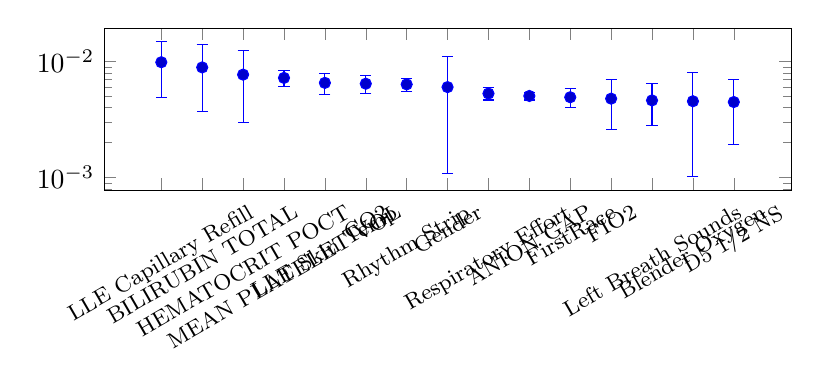
\begin{tikzpicture}
\begin{semilogyaxis} [
width=0.85\linewidth,
height=0.3\linewidth,
%log ticks with fixed point,
symbolic x coords={LLE Capillary Refill,BILIRUBIN TOTAL,HEMATOCRIT POCT,MEAN PLATELET VOL,LLE Skin Temp,CO2,Rhythm Strip,Gender,Respiratory Effort,ANION GAP,FirstRace,FIO2,Left Breath Sounds, Blender Oxygen,D5 1/2 NS},
xtick=data,
%ytick=data,
ymode=log, % Set y-axis to logarithmic scale
log basis y={10}, % Base 10 logarithm for the y-axis
xticklabel style = {font=\footnotesize, rotate=30},
]
\addplot+[only marks] plot[error bars/.cd, y dir=both, y explicit]
coordinates{
    (LLE Capillary Refill,0.00986033870379835) +- (0.0147661644336152,0.00495451297398151)
    (BILIRUBIN TOTAL,0.00889949693092115) +- (0.0126273414402402,0.00517165242160214) 
    (HEMATOCRIT POCT,0.00771484551610147) +- (0.0106733043693973,0.00475638666280566)
    (MEAN PLATELET VOL,0.00722791639121327) +- (0.0155413424057195,-0.00108550962329301)
    (LLE Skin Temp,0.00654834543779) +- (0.0117898135027299,0.00130687737285006)
    (CO2,0.00643982552509323) +- (0.0117188530496206,0.00116079800056584)
    (Rhythm Strip,0.0063570944708815) +- (0.0135076080519946,-0.00079341911023163)
    (Gender,0.0060215957123226) +- (0.007101505027428,0.00494168639721721)
    (Respiratory Effort,0.00529990635784179) +- (0.00995787056878017,0.000641942146903415)
    (ANION GAP,0.00505141865792101) +- (0.00971814564992059,0.000384691665921432)
    (FirstRace,0.00492530982150281) +- (0.00893863381241345,0.000911985830592171)
    (FIO2,0.00478955726231307) +- (0.00737036239483328,0.00220875212979286)
    (Left Breath Sounds,0.00462497034406318) +- (0.00745013982514881,0.00179980086297755)
    (Blender Oxygen,0.00454991688743892) +- (0.00556981498211942,0.00353001879275842)
    (D5 1/2 NS,0.00447869625451364) +- (0.00641773512494759,0.00253965738407969)
};
\end{semilogyaxis} 
\end{tikzpicture}